\documentclass[a4paper]{article}
\usepackage[utf8]{inputenc}
\usepackage[english,russian]{babel}
\usepackage{amsmath}
\usepackage{amssymb}
\usepackage{amsfonts}
\usepackage{graphicx}

\begin{document}

\section{Определение окна запуска в meet-and-greet}

Обозначения:
\begin{enumerate}
\item $r_1$ --- исходная орбита нашего спутника
\item $r_2$ --- орбита спутника-цели
\item $\omega(r)$ --- угловая скорость (радиан в секунду) на круговой орбите радиуса $r$
\item $\tau$ --- время перехода с орбиты $r_1$ на $r_2$
\item $T$ --- время начала маневра перехода
\item $\alpha(t)$ --- положение на орбите (полярный угол, в радианах) нашего спутника в момент времени $t$
\item $\beta(t)$ --- положение на орбите спутника-цели в момент времени $t$
\end{enumerate}

($T$ надо найти)

Чтобы попасть в спутник-цель, надо, чтобы в момент завершения перехода на орбиту, совпали положения спутников:$$\alpha(T+\tau)=\beta(T+\tau)\pm2\pi k,k\in\mathbb{Z}.$$

$$\alpha(T+\tau)=\alpha(T)+\pi=\alpha(0)+\pi+\omega(r_1)T$$

$$\beta(T+\tau)=\beta(0)+(T+\tau)\omega(r_2).$$

$$\alpha(T+\tau)-\beta(T+\tau)=$$
$$=\alpha(0)+\pi+\omega(r_1)T-\beta(0)-(T+\tau)\omega(r_2)=$$
$$T(\omega(r_1)-\omega(r_2))+(\alpha(0)+\pi-\beta(0)-\tau\omega(r_2))=$$
$$Tc_1+c_2.$$

Чтобы выполнилось условие попадания спутника в цель, надо чтобы выполнялось
$$Tc_1+c_2=2\pi k$$.

Обозначим $$z=\left\{\frac{c_2}{2\pi}\right\},$$ тогда $$c_2=2\pi q+z,\quad q\in\mathbb Z$$

Тогда, если положим $T$ таким, что $$\mbox{при } c_1>0: \quad Tc_1=2\pi-z\quad\Rightarrow\quad T=\frac{2\pi-z}{c_1},$$
$$\mbox{при } c_1<0: \quad Tc_1=-z\quad\Rightarrow\quad T=\frac{-z}{c_1},$$ то $T>0$ и выполнится условие:
$$2\pi-z+2\pi q+z=2\pi (q+1),\quad\mbox{ или }\quad -z+2\pi q+z=2\pi q,$$
и при этом $$T>0.$$

\section{Коррекция орбиты}

\textbf{Все это неправильно}

Обозначения:
\begin{enumerate}
\item $r$ --- радиус орбиты
\item $v$ --- линейная скорость движения спутника по орбите
\item $\omega$ --- угловая скорость движения спутника по орбите
\item $g(r)$ --- гравитационное ускорение на высоте $r$
\end{enumerate}

Когда спутник летит по круговой орбите, выполняется соотношение
$$g(r)=\frac{v^2}{r}.$$

Допустим, что мы хотим изменить линейную скорость движения спутника по орбите на $\Delta v_\tau$. Тогда необходимо будет придать дополнительное нормальное ускорение:
$$g(r)+\Delta v_n=\frac{(v+\Delta v_\tau)^2}r.$$

Таким образом, $$\Delta v_n=\frac{(v+\Delta v_\tau)^2}r-g(r).$$

Посчитаем, какую линейную скорость надо сообщить спутнику, чтобы изменить его угловую скорость на $\Delta \omega$.

Период обращения спутника можно выразить двумя способами:
$$T=\frac{2\pi}{\omega}=\frac{2\pi r}{V},$$
откуда
$$v=r\omega,$$
и
$$\Delta v=r\Delta\omega.$$

Таким образом, для изменения угловой скорости на $\Delta\omega$ необходимо изменить линейную скорость на $\Delta v$.

Чтобы <<догнать>> другой спутник на орбите, отстоящий на угол $\Delta\phi$, необходимо в течение секунды изменить угловую скорость на $\Delta\omega$.

\section{Активная компенсация ошибки}

\begin{enumerate}
\item $x(t)$ --- положение (радиус-вектор) нашего спутника в момент времени $t$
\item $y(t)$ --- положение спутика-цели в момент времени $t$
\item $x_0$ --- начальное положение спутника
\item $y_0$ --- начальное положение спутника-цели
\item $v_x$ --- начальная скорость спутника (вектор)
\item $v_y$ --- начальная скорость спутника-цели (вектор)
\item $a_x$ --- гравитационное ускорение спутника (в начальный момент времени)
\item $a_y$ --- гравитационное ускорение спутника-цели (в начальный момент времени)
\item $\alpha$ --- ускорение спутника, вызванное работой двигателей
\end{enumerate}

В течение одной секунды движение спутников описывается уравнениями:
$$x(t)=x_0+v_xt+\frac12a_xt^2+\frac12\alpha t^2,$$
$$y(t)=y_0+v_yt+\frac12a_yt^2.$$

К концу первой секунду спутники будут иметь скорости
$$v'_x=v_x+a_xt+\alpha,$$
$$v'_y=v_y+a_yt.$$

Необходимо выбрать $\alpha$ таким образом, чтобы быть как можно ближе к цели. Будем искать $\alpha$ исходя из той ситуации, которая будет к концу первой секунды. На следующей секунде все расчеты необходимо будет повторить.

Если $\alpha$ выбрать таким образом, чтобы минимизировать $\left|x(1)-y(1)\right|$, то это приведет к тому, что будет значительная разница скоростей $v'_x, v'_y$, и на следующей секунде спутник наберет большую скорость, и начнется резонасная осцилляция скорости спутника, которая в конце приведет к тому, что у спутника не хватит топлива на очередную коррекцию.

Поэтому, будем выбирать $\alpha$ таким образом, чтобы минимизировать как погрешность положения, так и погрешность скорости:
$$\left|x(1)-y(1)\right|^2+\left|v'_x-v'_y\right|^2\rightarrow\min.$$

Распишем:
$$\left\{
\begin{array}{rcl}
x(1)-y(1)&=&\underbrace{x_0-y_0+v_x-v_y+\frac12a_x-\frac12a_y}_{p}+\frac12\alpha\\
v'_x-v'_y&=&\underbrace{v_x-v_y+a_x-a_y}_{q}+\alpha
\end{array}\right.
$$
$$\left\{
\begin{array}{rcl}
x(1)-y(1)&=&p+\frac12\alpha\\
v'_x-v'_y&=&q+\alpha
\end{array}\right.$$

Таким образом, задача нахождения $\alpha$ записывается в виде
$$(p_x+\frac12\alpha_x)^2+(p_y+\frac12\alpha_y)^2+(q_x+\alpha_x)^2+(q_y+\alpha_y)^2\rightarrow\min,$$
где $p_x,p_y,q_x,q_y,\alpha_x,\alpha_y$ --- $x$- и $y$-компоненты векторов.

Отдельно минимизируем выражения, зависящие от $\alpha_x$ и $\alpha_y$:

$$\left\{
\begin{array}{rcl}
(p_x+\frac12\alpha_x)^2+(q_x+\alpha_x)^2&\rightarrow&\min\\
(p_y+\frac12\alpha_y)^2+(q_y+\alpha_y)^2&\rightarrow&\min\\
\end{array}\right.$$

Рассмотрим выражение, зависящее от $\alpha_x$:
$$(p_x+\frac12\alpha_x)^2+(q_x+\alpha_x)^2\rightarrow\min$$

Перепишем его в виде
$$\alpha_x^2(\frac14+1)+\alpha_x(p_x+2q_x)+(p_x^2+q_x^2)\rightarrow\min$$

Это выражение задает параболу с ветвями, уходящими вверх. Минимум это параболы --- вершина параболы, соответствующая значению
$$\alpha_x=-\frac{p_x+2q_x}{\frac52}=-\frac45q_x-\frac25p_x.$$

Аналогично, $$\alpha_y=-\frac45q-\frac25p.$$

Таким образом,
$$\alpha=-\frac45q-\frac25p,$$
где
$$p=x_0-y_0+v_x-v_y+\frac12a_x-\frac12a_y,$$
$$q=v_x-v_y+a_x-a_y.$$

График зависимости расстояния от спутника до цели от времени при использовании активной компенсации:

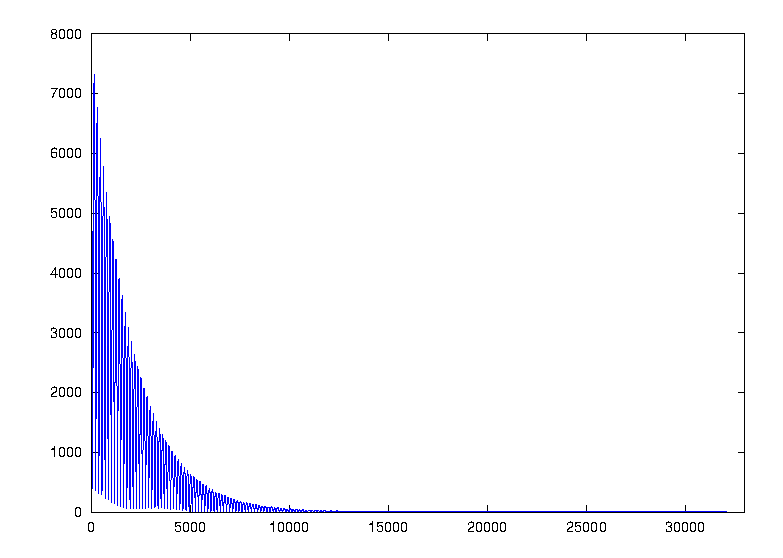
\includegraphics[width=\textwidth]{active-chase}

\end{document}